\clearpage
\subsection{実習2-2 課題実験}
\begin{itemize}
	\item プログラム\ref{ex22-block}は変電圧測定プログラムである.これのようにNの値を11に,カウンタ変数を2で除することで0\,\rm{V}から5\,\rm{V}まで0.5\,\rm{V}刻みで出力電圧を計測することが可能となる.
	\item 実行した後のフロントパネルを\wfig{ex22-flont}に示す.また,\weq{soutaigosa}に基づいて計算した相対誤差を\wtab{fivegosa}に示す.
表からもわかるように0\,\rm{V}の際の相対誤差が飛び抜けて大きいことが読み取れる.	
	\item Excel を用いて計算したRMSEを\wtab{RMSE}に示す\cite{lm-evaluation}.
	\item RMSEの計算式は\weq{lm-evaluation},Excelでは\weq{eRMSE}で計算した.
\end{itemize}

\begin{align}
RMSE&=\sqrt{\frac{1}{n}\sum_{i=1}^{n}(y_{i}-\hat{y_{i}})^{2}}\label{eq:lm-evaluation}\\
y_{i}:観測値(n個)\quad&\qquad\hat{y_{i}}:計算値(n個)\nonumber\\
RMSE&=SQRT(1/11)*SQRT(SUM(\overline{X_{i}}^{2}))\label{eq:eRMSE}\\
\overline{X_{i}}&:X_{i}での差(誤差)\nonumber
\end{align}

\begin{figure}[h]
\centering
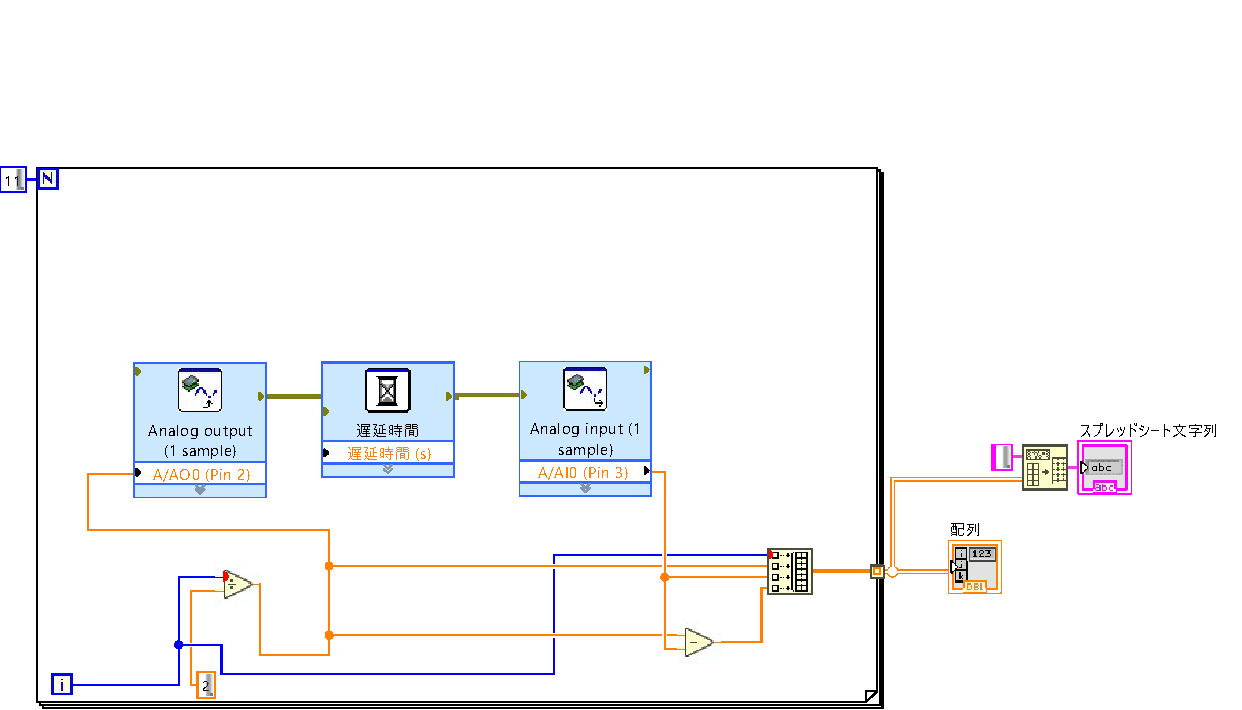
\includegraphics[scale=0.5]{./fig/ex22-block.pdf}\\
\useMycounter[\label{ex22-block}]出力電圧変化測定時のブロックダイアグラム
\end{figure}
\begin{figure}[h]
\centering
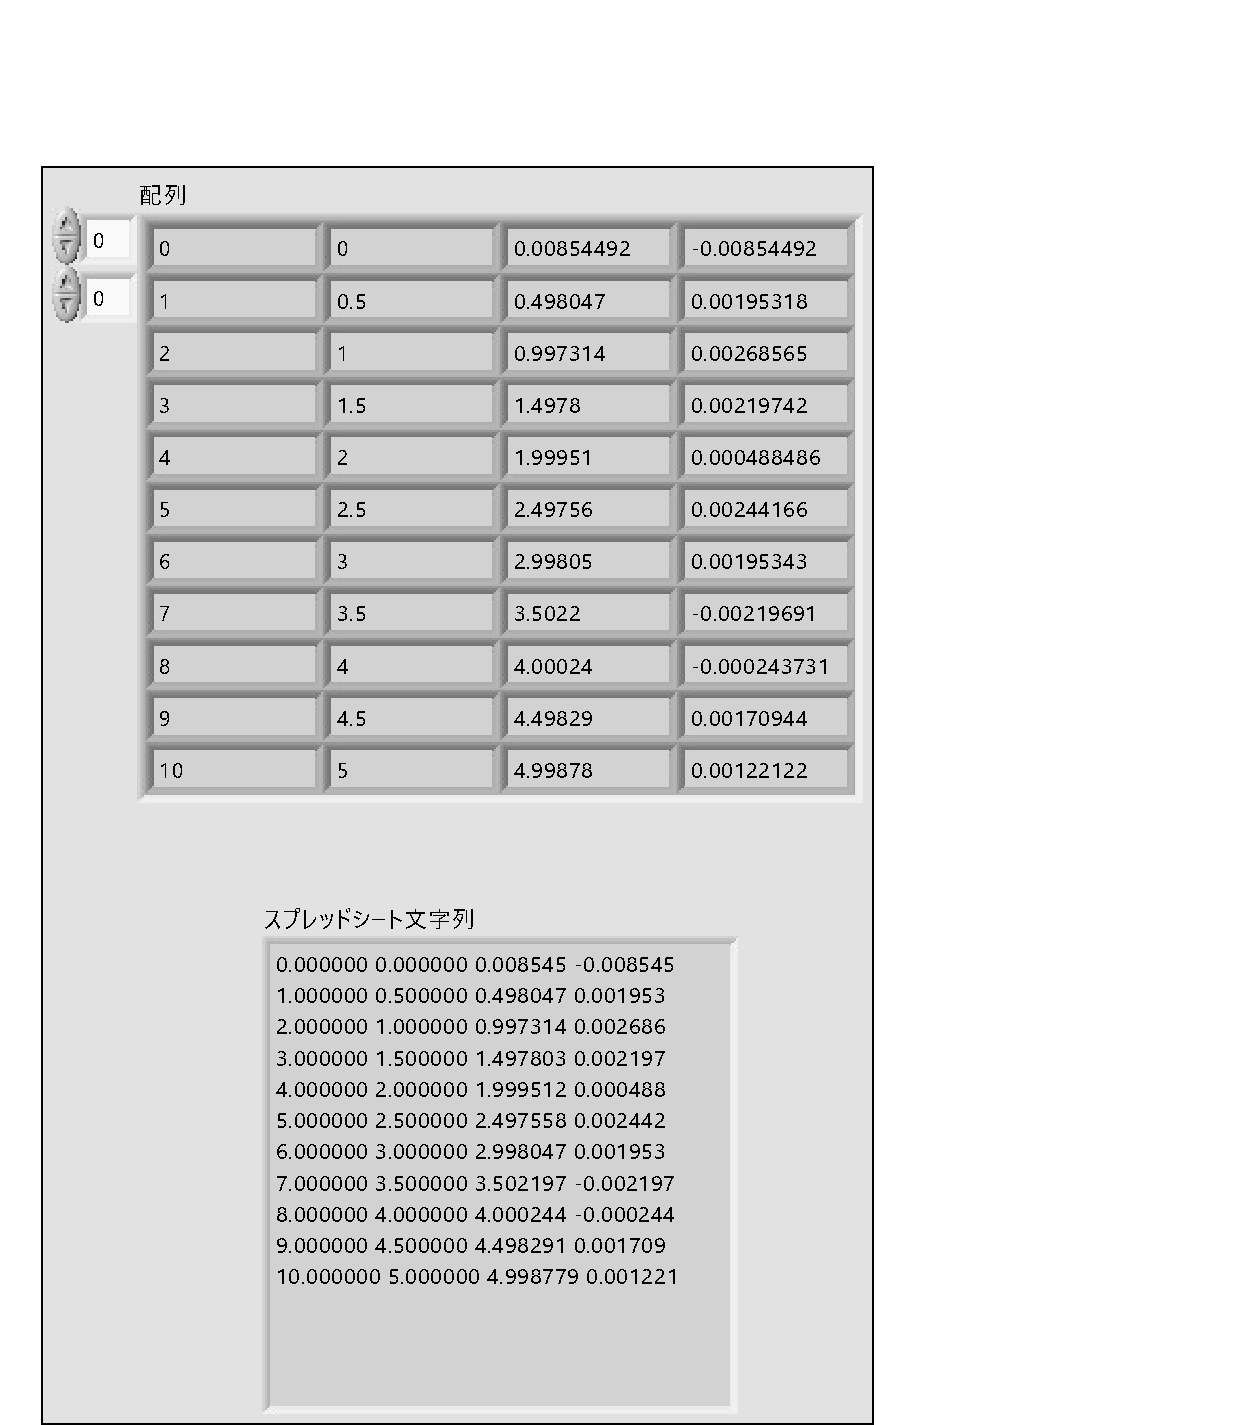
\includegraphics[scale=0.5]{./fig/ex22-flont.pdf}
\caption{出力電圧変化測定時のフロントパネル}
\label{fig:ex22-flont}
\end{figure}

\begin{table}[h]
\begin{minipage}[c]{0.5\hsize}
\centering
\caption{電圧変化測定時の相対誤差}
\label{tab:fivegosa}
\begin{tabular}{cc}
\hline
電圧[\rm{V}]  & 相対誤差[\rm{V}]\\
\hline
0   & 0  \\
0.5 & 0  \\
1   & -1 \\
1.5 & -1 \\
2   & -2 \\
2.5 & -3 \\
3   & -3 \\
3.5 & -3 \\
4   & -4 \\
4.5 & -4 \\
5   & -5 \\
\hline
\end{tabular}
\end{minipage}
\begin{minipage}[c]{0.5\hsize}
\centering
\caption{電圧変化測定時のRMSE}
\label{tab:RMSE}
\begin{tabular}{cc}
\hline
電圧[\rm{V}]  & 二乗平均平方根誤差[\rm{V}]  \\
\hline
0   & 0.002576414 \\
0.5 & 0.000956997 \\
1   & 0.000809859 \\
1.5 & 0.001030566 \\
2   & 0.000515283 \\
2.5 & 0.000367844 \\
3   & 0.000221008 \\
3.5 & 0.0000735688 \\
4   & 0.000441413 \\
4.5 & 0.000147439 \\
5   & 0.000368145\\
\hline
\end{tabular}
\end{minipage}
\end{table}